\documentclass{article}
\usepackage[nonatbib]{project}
\usepackage{watml}

\usepackage[normalem]{ulem}
\usepackage{setspace}
% use Times
\usepackage{times}
% For figures
\usepackage{graphicx} % more modern
%\usepackage{epsfig} % less modern
%\usepackage{subfig}

% path to figure folder
\graphicspath{{../fig/}}

% bib file for references
\addbibresource{project.bib}


\title{CS 480/680 Project: Predicting 6 Vital Plant Traits}

\author{
	Jiaze Xiao \\
	University of Waterloo\\
	Waterloo, ON, N2L 3G1 \\
	\texttt{j76xiao@uwaterloo.ca}
}

\begin{document}
\maketitle

\begin{abstract}
	This project explores the prediction of 6 vital plant traits using a combination of ancillary data and image features. A pre-trained DinoV2 model is employed to extract image features, which are combined with ancillary data to train CatBoostRegressors. The project demonstrates the potential of integrating deep learning and traditional regression techniques for plant trait prediction.
\end{abstract}

\section{Introduction}
Predicting plant traits is crucial for understanding plant health and optimizing agricultural practices. Traditional approaches rely heavily on manual measurements, which are time-consuming and prone to error. Recent advancements in machine learning, particularly in computer vision, offer the potential to automate and enhance the accuracy of these predictions.

This project focuses on predicting 6 vital plant traits using a combination of ancillary data (such as soil and climate information) and image features extracted from plant photographs. A robust prediction model is built by leveraging a pre-trained DinoV2 model for feature extraction and combining it with 6 CatBoostRegressors. \Cref{fig:targets} shows the distribution of the targets I are predicting.

\begin{figure*}[h]
	\centering
	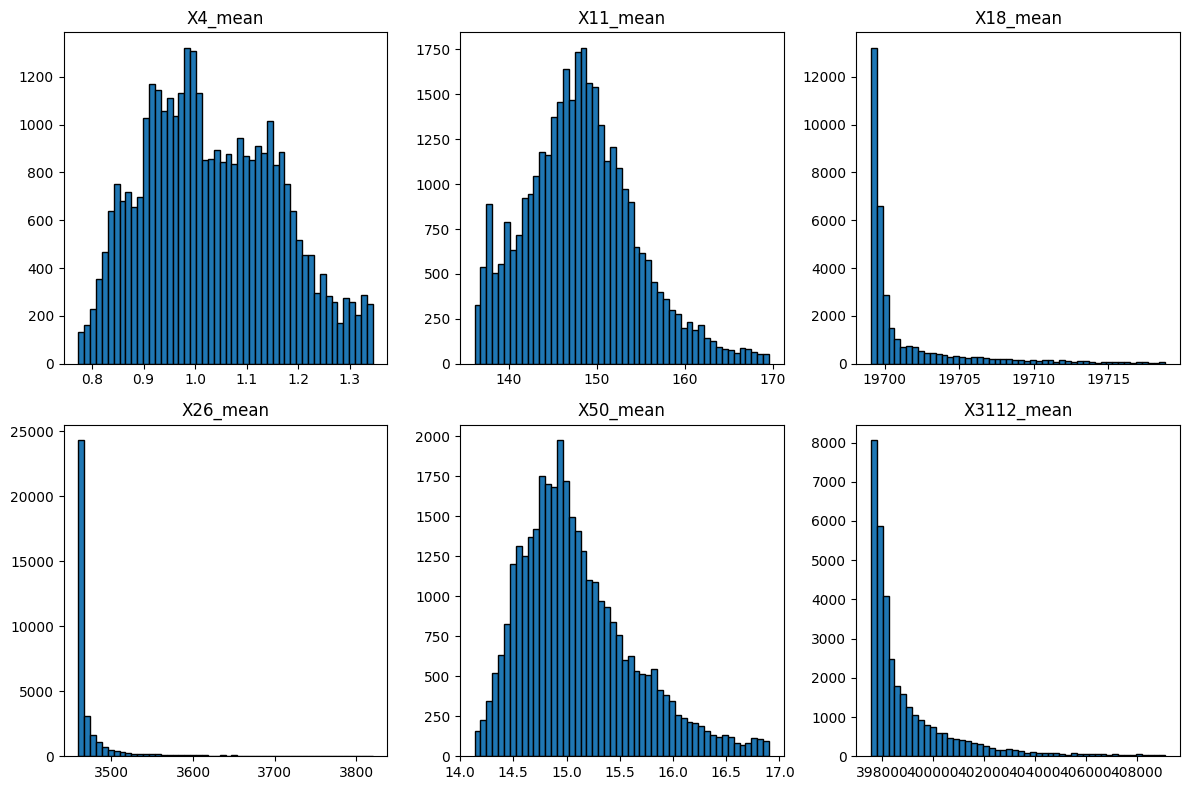
\includegraphics[scale=0.4]{targets.png}
	\caption{The 6 vital plant traits used for training with outliers removed.}
	\label{fig:targets}
\end{figure*}

\section{Related Works}

\subsection{Experiments with End-to-End Models}
In addition to the feature extraction approach, I experimented with end-to-end models where images are directly fed into a neural network alongside ancillary data. I implemented two versions of the PlantTraitPredictionModel: one using a structured self-attention mechanism and another using a simpler fully connected approach. Both models utilized a ResNet, ConvNeXT or Vision Transformer (ViT) for image feature extraction.

I applied various data augmentations during training, including random flips, rotations, and color jittering, to improve generalization. Additionally, I tested multiple hyperparameter configurations, including different learning rates, optimizers, and fully connected layer sizes. Despite these efforts, the highest R2 score achieved by these models is less than 0.4, with most results falling between 0.1 and 0.4.

\subsection{Experiments with Feature Extraction and CatBoost}
In contrast to the end-to-end models, I explored an alternative approach where features are first extracted from images using pre-trained models and then fed into regression models such as CatBoost and XGBoost. This methodology is inspired by the approach of \citet{korotas2024}, who successfully combined DinoV2-extracted image features with ancillary data to predict plant traits.

Initially, I used ConvNeXT for feature extraction, followed by CatBoost regression. However, the performance did not show a substantial improvement compared to the end-to-end models, with only a marginal increase in R2 scores. This result suggests that while ConvNeXT is effective for classification tasks, it may not be as optimized for feature extraction in the context of plant trait prediction.

A significant breakthrough came when I employed DINOv2, a variant of the Vision Transformer (ViT) specifically designed for robust feature extraction by \citet{DINOv2}. Unlike traditional ViT models, which are primarily focused on classification tasks, DINOv2 is tailored to produce high-quality, generalizable features that can be effectively used for downstream tasks such as regression.

The use of DINOv2 for feature extraction, followed by regression with CatBoost or XGBoost, led to a substantial improvement in model performance. The R2 scores consistently exceeded 0.46, highlighting the advantage of using a model specialized in feature extraction. This improvement underscores the importance of selecting the right feature extraction model for the task at hand.

\begin{table}[h]
	\centering
	\caption{R2 Scores on Test Set: End-to-End Models vs. Feature Extraction with CatBoost.}
	\begin{tabular}{lcc}
		\toprule
		Model                                         & Best R2 Score    & Average R2 Score \\
		\midrule
		End-to-End with ViT                           & 0.19441          & 0.16990          \\
		End-to-End with ConvNeXT                      & 0.32319          & 0.28040          \\
		End-to-End with ResNet                        & 0.26927          & 0.19710          \\
		Feature Extraction with ConvNeXT and CatBoost & 0.26324          & 0.26324          \\
		Feature Extraction with DINOv2 and XGBoost    & 0.39543          & 0.39543          \\
		Feature Extraction with DINOv2 and CatBoost   & \textbf{0.46085} & \textbf{0.45932} \\
		\bottomrule
	\end{tabular}
	\label{tab:r2-comparison}
\end{table}


\section{Main Results}
\subsection{Preprocessing}
The feature extraction approach begins with preprocessing the ancillary data, where outliers are removed, and features are normalized using a \texttt{StandardScaler}. The image features are extracted using the DINOv2 model, which are then combined with polynomial-transformed ancillary features to create a comprehensive dataset for training. The entire process took approximately 3 hours, with 2 hours dedicated to feature extraction and 1 hour for model training.

Polynomial transformations are used to enhance the model's ability to capture complex interactions between the features. In this context, the ancillary data includes variables such as soil pH, moisture, and other environmental factors, which can have non-linear relationships with the target traits. It allows the model to consider not only the individual features but also the interactions between them.

\subsection{Feature Extraction}
The DINOv2 model, specifically tailored for robust feature extraction, is employed to extract meaningful features from the plant images. These features are then combined with polynomial-transformed ancillary data, which allowed the model to capture higher-order interactions between the features, ultimately improving the model's predictive performance.

\subsection{Model Training}
For each of the 6 target traits, a separate CatBoostRegressor is trained using the combined features. CatBoost is a gradient boosting algorithm that is particularly well-suited for structured data, such as the one used in this project. Here are the resons for choosing CatBoost:

\begin{itemize}
	\item Fast Training on GPUs: CatBoost supports GPU acceleration, which significantly reduces training time when dealing with large datasets, like the combination of image and ancillary features in this project.
	\item Robustness to Overfitting: \citet{CatBoost} highlighted CatBoost's effectiveness in handling categorical data and its robustness to overfitting, making it an ideal choice for structured data tasks.
\end{itemize}

The parameters chosen for CatBoost (e.g., 2000 iterations, a learning rate of 0.085) are selected based on a balance between computational efficiency and model performance. The performance of each model is evaluated using the R2 score, the results are summarized in \Cref{tab:r2-scores}.

\begin{table}[h]
	\centering
	\caption{Model performance on the validation set, measured by R2 score. (SEED=6)}
	\begin{tabular}{lc}
		\toprule
		Trait       & R2 Score \\
		\midrule
		X4\_mean    & 0.513    \\
		X11\_mean   & 0.473    \\
		X18\_mean   & 0.628    \\
		X26\_mean   & 0.272    \\
		X50\_mean   & 0.366    \\
		X3112\_mean & 0.463    \\
		\midrule
		average     & 0.452    \\
		\bottomrule
	\end{tabular}
	\label{tab:r2-scores}
\end{table}

The models showed varying levels of accuracy across different traits, with the highest R2 score being 0.628 for X18\_mean and the lowest being 0.272 for X26\_mean. This variation suggests that some traits are more predictable based on the available data and features than others.

\subsection{Potential Improvements}
While the overall performance is strong, there are areas for improvement:
\begin{itemize}
	\item \textbf{Trait-Specific Regressors}: Currently, the same regression model (CatBoost) is used for all traits, which may not be optimal. For example, the traits X26\_mean and X50\_mean had lower R2 scores, suggesting that a different regressor, or a more specialized model, might perform better for these traits. Exploring other regression techniques, such as XGBoost or even neural network-based models, could yield better results for these specific traits. However, this would require additional time and resources, which may not be justified given the already satisfactory overall R2 score.
	\item \textbf{Hyperparameter Tuning}: Further fine-tuning of the CatBoost parameters and outlier quantiles could improve performance, particularly for the traits that are currently underperforming.
	\item \textbf{Feature Selection}: Conducting a more thorough feature selection process could help in identifying which features (including polynomial terms) are most predictive for each trait, leading to more efficient models.
\end{itemize}

\subsection{Robustness of Results}
To ensure the robustness of our results, I evaluated the models using different random seeds. \Cref{tab:r2-scores-across-seeds} shows the average R2 scores obtained with various seeds. The consistency across different seeds indicates that the models are stable and not overly sensitive to the randomness in data splitting or model initialization.

\begin{table}[h]
	\centering
	\caption{R2 scores on the test set across different random seeds.}
	\begin{tabular}{lc}
		\toprule
		Seed   & Average R2 Score \\
		\midrule
		6      & \textbf{0.46085} \\
		42     & 0.45518          \\
		911    & 0.45638          \\
		1234   & 0.45830          \\
		10086  & 0.45882          \\
		6666   & 0.45740          \\
		666666 & 0.45587          \\
		\bottomrule
	\end{tabular}
	\label{tab:r2-scores-across-seeds}
\end{table}


\section{Conclusion}
This project demonstrates the effectiveness of integrating deep learning-based feature extraction with traditional regression models for predicting plant traits. By leveraging a pre-trained DINOv2 model, specifically designed for high-quality feature extraction, and combining these features with polynomial-transformed ancillary data, a significant improvement in prediction accuracy is achieved.

The results highlight several key points:

\begin{itemize}
	\item \textbf{Feature Extraction Matters}: The choice of feature extraction model (DINOv2) significantly influenced the model's performance, outperforming more conventional architectures like ConvNeXT and ResNet in this context.
	\item \textbf{Hybrid Approach}: Combining image-based features with ancillary data through polynomial transformations captures more complex interactions, leading to better predictive performance.
	\item \textbf{Model Stability}: The consistent R2 scores across different random seeds indicate that the model is robust and generalizable.
	\item \textbf{Exploration of Trait-Specific Models}: While the current approach uses the same regression model for all traits, future work could explore using different models tailored to specific traits, particularly those that are currently underperforming.
\end{itemize}

Overall, this project contributes to the ongoing efforts to automate and enhance plant trait prediction, with potential applications in agriculture and environmental monitoring.

\newpage

\nocite{*}
\printbibliography[title=References]


\end{document}